% !TeX spellcheck = en_US
% !TeX root = main.tex

\section{Navigation and Organisation}
\subsection{Card Sorting}
% Reflect on the success of the Card Sorting design activity you did in Week 4
% Include the testing plan you developed for the activity
% Include photos you took of the activity running
% What feedback did you get and how did it inform your early content organisation decisions?
% Which organisation systems will you use in your website and why?

\subsubsection{The Plan}
To begin there were three main areas of content were identified: Git Reference Summary, Main storyline/tutorial, Interactive Quiz. These areas were then assigned a rank and associated keywords:
\begin{itemize}
	\item\textbf{Git Reference Summary}
	\begin{itemize}
		\item Shows all the commands and a basic overview of what they do
		\item This will be visited most by people coming back because they forgot something or wanted to know more outside of the main storyline
		\item \textbf{Rank:} 2
		\item \textbf{Keywords:} Advanced, Reflection, Quick
	\end{itemize}
	\item\textbf{Main storyline/tutorial}
	\begin{itemize}
		\item This will be most frequently visited by new comers and people just visiting the site
		\item \textbf{Rank:} 1
		\item \textbf{Keywords:} Beginner, Interesting, Interactive
	\end{itemize}
	\item\textbf{Interactive Quiz}
	\begin{itemize}
		\item Some of this will also be embedded inside the storyline
		\item People wanting a challenge and to learn more
		\item \textbf{Rank:} 3
		\item \textbf{Keywords:} Self Learning, Interactive, All Levels
	\end{itemize}	
\end{itemize}

For this survey I chose to go with an Open Card Sort because I wanted to observe how they thought about grouping and what is easier or more important to sort before arriving at a final decision. After the users had finished with sorting the cards, a couple of follow up questions/discussions would be had around why they named the groups they did.

\subsubsection{Execution}
In order to execute the card sorting, Trello was used for the physical moving of cards around. This decision was made because it best allows people to move the cards around like they would physically, while still providing them with the easy of changing the names of the groups.

\subsubsection{Results}
\begin{note}{Person 1}
	\begin{figure}[H]
		\centering
		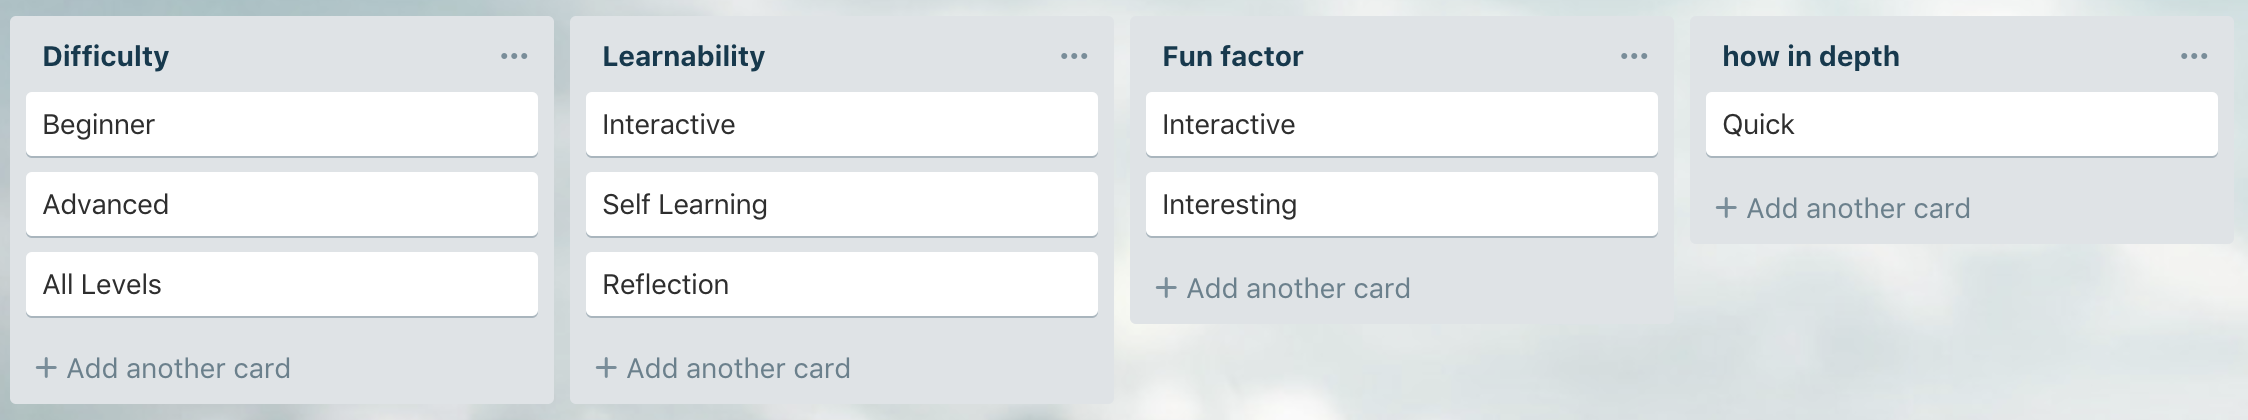
\includegraphics[width=\linewidth]{card1}	
		\caption{Person 1's Card Sorting Result}
	\end{figure}

	How did you group the tags?
	\begin{leftbar}
		Beginner and advanced are varying difficulties, I don't know if that is something I can choose. All levels are associated, can I filter by difficulty level on the side.\\\\
		Grouped them because the concepts are the same, but on the site I wouldn't expect beginner and advance to be together.
	\end{leftbar}

	How did you name the groups?
	\begin{leftbar}
		\begin{itemize}
			\item Difficulty
			\begin{itemize}
				\item When you play a video game you pick your difficulty level
			\end{itemize}
			\item Learnability
			\begin{itemize}
				\item Self learning, learnability makes sense
				\item Interactive is key to learning
				\item Reflection is key to learning, gauge how successful you were
			\end{itemize}
			\item Fun Factor
			\begin{itemize}
				\item Interactive website's are fun, reading a static page can be quite passive and boring
				\item It's interesting because I am curious and it feels more tactile
			\end{itemize}
			\item How in Depth (\textit{mean not very in depth})	
			\begin{itemize}
				\item I would go through the site really quickly
				\item So the level of detail in the website is probably really shallow
			\end{itemize}
		\end{itemize}
	\end{leftbar}
\end{note}

\begin{note}{Person 2}
	\begin{figure}[H]
		\centering
		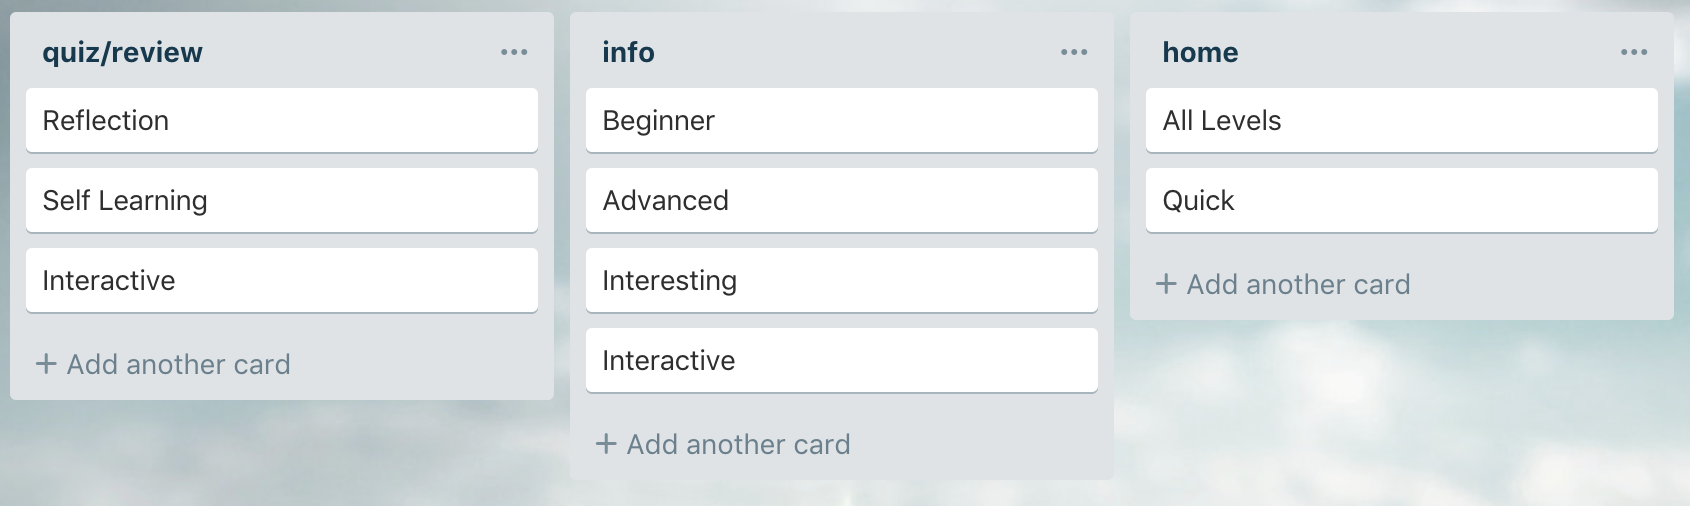
\includegraphics[width=\linewidth]{card2}	
		\caption{Person 2's Card Sorting Result}
	\end{figure}

	How did you group the tags?
	\begin{leftbar}
		Beginner and advanced are linked and interesting is cool\\\\
		All Levels and Quick are navigation type\\\\
		Reflection/SL/Interactive seem like quizzing	
	\end{leftbar}
	
	How did you name the groups?
	\begin{leftbar}
		\begin{itemize}
			\item Quiz/Review
			\begin{itemize}
				\item Reflection/SL is like looking back at what you learnt
				\item Looking back
			\end{itemize}
			\item Info
			\begin{itemize}
				\item Looking at Beginner and Advanced and interactive is like the middle of where you go
				\item Middle man of the navigation
			\end{itemize}
			\item Home
			\begin{itemize}
				\item They seem like navigation and be able to go through the site
			\end{itemize}
		\end{itemize}
	\end{leftbar}
\end{note}

\subsubsection{Summary}
When it came to grouping the content together both Person 1 and Person 2 grouped elements together with an understanding of the level of difficulty different tags have. Since both users mentioned this first it can be assumed this is the primary concern or forefront of user thought. Person 1 also created a card group based on interactivity, Person 2 also mentioned that there are cards that are related to interactivity. Therefore is can be assumed that users are also grouping based on how much static an element is and how interactive it is.\\\\
From these content can be broken up into three main sections:
\begin{description}
	\item[Main Homepage:] This page is the main area where the user will learn the basics and be interested to learn more. This site will be majority static content.
	\item[Reference Sheet:] This page will be just a bunch of commands and the usage/description of the commands. This site will also be a static based site.
	\item[Quizzes:] The quizzes will be used for the user to recap the knowledge they have learnt through the site. This site will be interactive and only supported on browsers which support a wide range of interactivity.
\end{description}\vspace{1em}
These three pages help to break up the content through the two categories identified in the card sorting. Main Homepage and Reference Sheet allow for two different difficulty levels (beginner and advanced respectively), while delivering primarily non-interactive. The Quizzes page covers all difficulty level with the user specifying what difficulty level they want to be tested on. The Quizzes page will also provide a user interactive approach where all content displayed on the screen is based on interactions made by users.


\subsection{Navigation Systems}
% What were the key things you learned from your Navigation Systems group discussion?
% Write a brief response of your own to the guiding questions for this group discussion
% Which navigation systems will you use in your website and why?
A lot of the shown ``correct'' styles of navigation systems followed a similar style and placement. A lot of ``incorrect'' styles were outside the norm of having common elements. These elements are:
\begin{itemize}
	\item A main banner which include a general logo and quick navigation links underneath
	\item Most of the examples also used an inner page navigation panel on the left for filtering content on the current page	
\end{itemize}\vspace{1em}
Reflecting on the themes and the presentation styles used across websites that are considered good design, a similar layout will be used for this website. However slight modifications will be made to suit a scrolling storyline layout. To increase screen size and make the website appear more story like, the main logo will be reduced to be inline with the primary navigation menu. A side navigation menu will be created but it will be semi-hidden for a majority of the website and only showing itself when the mouse interacts with the shown tip.


\subsection{Site Map}
% todo[inline]{Need to add more here}
% Draw a site map that visualises the navigation flow of your website
% Include any internal (between pages) and external links
% Storyboard how one of your personas will navigate your website
\begin{figure}
	\centering
	\begin{tikzpicture}[node distance=2cm,thick,every node/.style={scale=0.8}]
		\node (main) [page] {Home Page};
		\node (menu) [menu, below of=main] {Main Navigation Bar};
		\node (quiz) [page, right of=menu,xshift=3cm] {Quizzes Page};
		\node (about) [page, below of=quiz] {About Page};
		\node (refs) [page, below of=about] {References Page};
		
		\node (innerMenu) [menu, left of=menu,xshift=-3cm] {Inner Page Menu};
		
		\node (externalGit) [page, right of=refs,xshift=3cm] {Official Git Documentation};
		
		\node (internal) [group, fit=(main) (menu) (refs) (quiz) (about) (innerMenu),label={Internal Links},scale=1.25] {};
		
		\draw [arrow] (main) -- (menu);
		\draw [arrow] (menu) -- (refs);
		\draw [arrow] (menu) -- (quiz);
		\draw [arrow] (menu) -- (about);
		\draw [->] (main) -- (innerMenu);
		\draw [->] (refs) -- (externalGit);
		\draw [->] (main) -- node [midway,above,rotate=-22]{Take the Quiz} (quiz);
	\end{tikzpicture}
	\caption{Site Map Navigation}\label{fig:sitemap}
\end{figure}

\subsubsection{Site Map Navigation}
The site map design is shown in Figure~\ref{fig:sitemap}, here the user will enter the site via the ``Home Page'' which will be the main story page. Then to navigate they can chose to navigate through the home page using the ``Inner Page Menu'' or via scrolling. The other main navigation feature will the be top bar which can be used to navigate to the other pages within the site (``Quizzes Page'', ``About Page'', ``References Page''). From these pages, the same navigation element will exist allowing the user to navigate back or to other pages as they see required.\\\\

There will be small link at the bottom of the home page what will direct the user to the quizzes page, this symbolises that they have all the knowledge they require and it is time to see if they really learnt as much or need to go back through and understand it much more clearly.


\subsection{Visual Organisation}
% What were the key things you learned from you Visual Organisation group discussion?
% Write a brief response of your own to the guiding questions for this group discussion

\begin{figure}
	\centering
	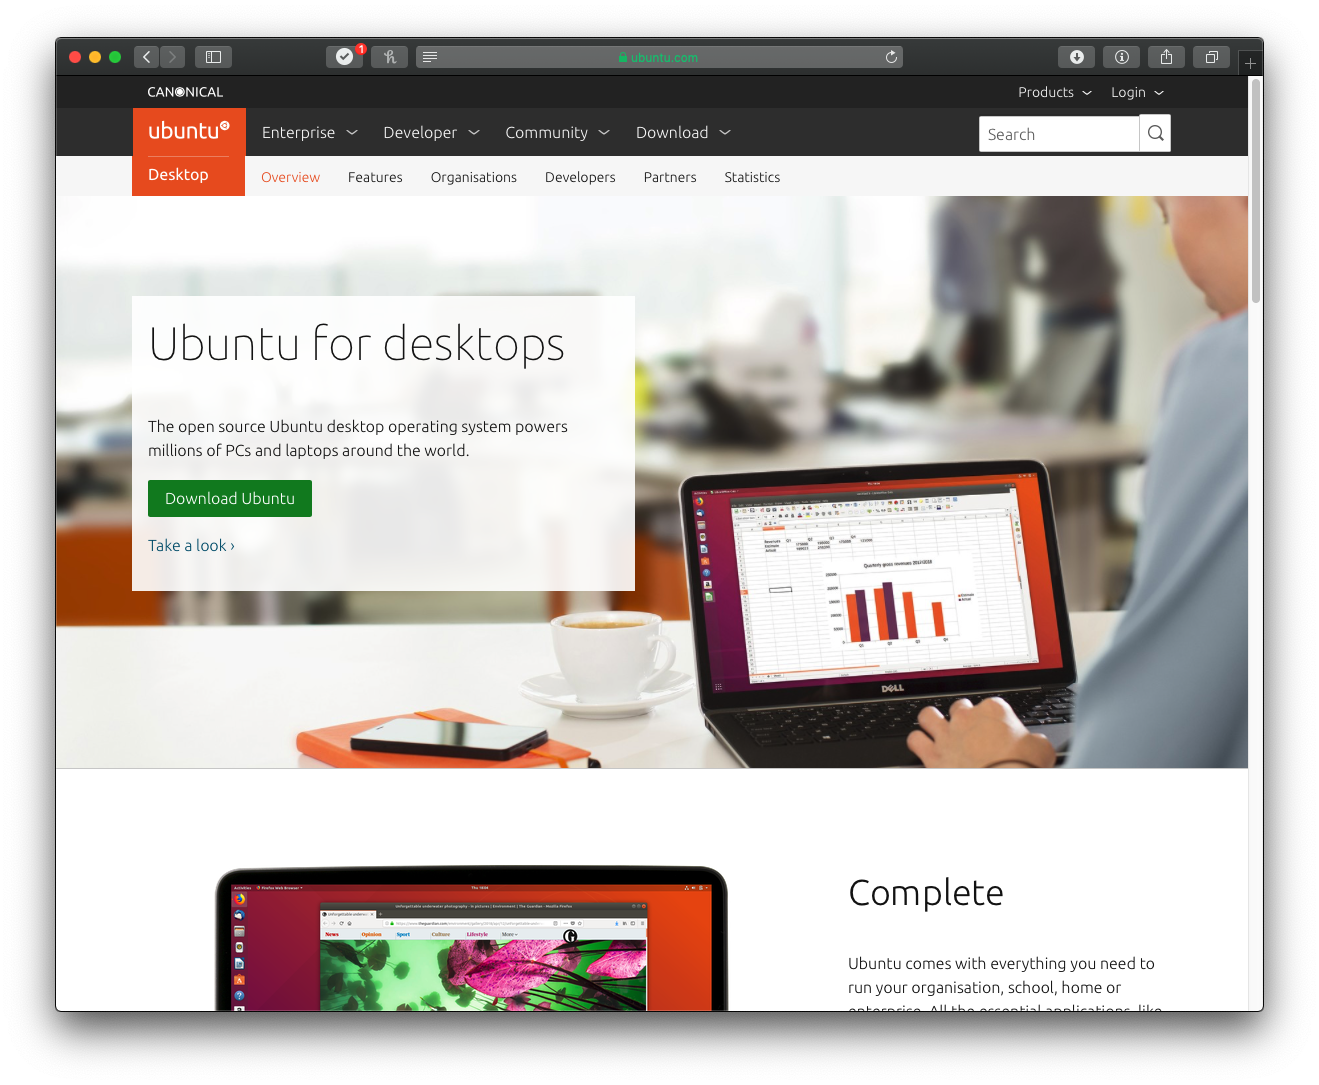
\includegraphics[width=\linewidth]{ubuntu}
	\caption{Screenshot of Ubuntu Desktop webpage}\label{fig:ubuntu}
\end{figure}

The example site picked for the visual organisational layout is the Ubuntu Desktop webpage (Figure~\ref{fig:ubuntu}). This site incorporates a lot of good design choices and creates a very pleasant user experience through its choice in positioning and colors.

\subsubsection{Spacing}
The page utilises a lot of spacing around elements to signify the beginning and ending of different sections and content. And pictures are used to help create this space without making the space seem stretched out or the significance of ``white space''.

\subsubsection{Colours and Fonts}
Ubuntu has used a very basic colour palette here, simply just black and white with orange as a primary colour. The use and choice of colour has resulted in the images having a really attention drawn in factor and the text combined with the font choice, is easy and delightful to read. A user is draw to the picture foremost and then curiosity about what they are looking at draws them into the text to find out more. The styling of the text creates a calm and informal attitude which invites readers to only view the information they think is relevant.

\subsubsection{Alignment and Layout}
The webpage appears to use a three column approach where either content is split across three columns, or the image consumes two columns and text is floated left or right of the image. However due to the use of spacing, this column structure is not strict and instead boosts the appearance of a relax and informal presentation.

\subsubsection{Weight}
Ubuntu has taken a none-traditional approach to weight in web design by not so much assigning weighting to how bold or coloured the text is. Instead an approach of providing spacing and increased font size is favoured, however font weighting is still used. This primarily puts focus around the user seeing the larger text and the proceeding white space around it as a reference for the weight of a piece of text. This unique approach has provided Ubuntu with the relaxed and informal vibe that appears to be the design goal behind the entire site.


\subsection{Interactivity and Functionality}
% Draw wireframes for each type of page in your website (i.e. if you have 5 pages that function very similarly, you only need to draw 1 wireframe)
% These can be derived from the same mockups you produced for Paper Prototyping
% Add annotations to describe:
% - how each interactive element functions
% - how they are designed to engage your specific target audience
% - how they are designed to strengthen the educational content
% - and how you think it will be implemented at this stage (HTML, CSS or JavaScript)

\subsubsection{Title Page}
\begin{figure}
	\centering
	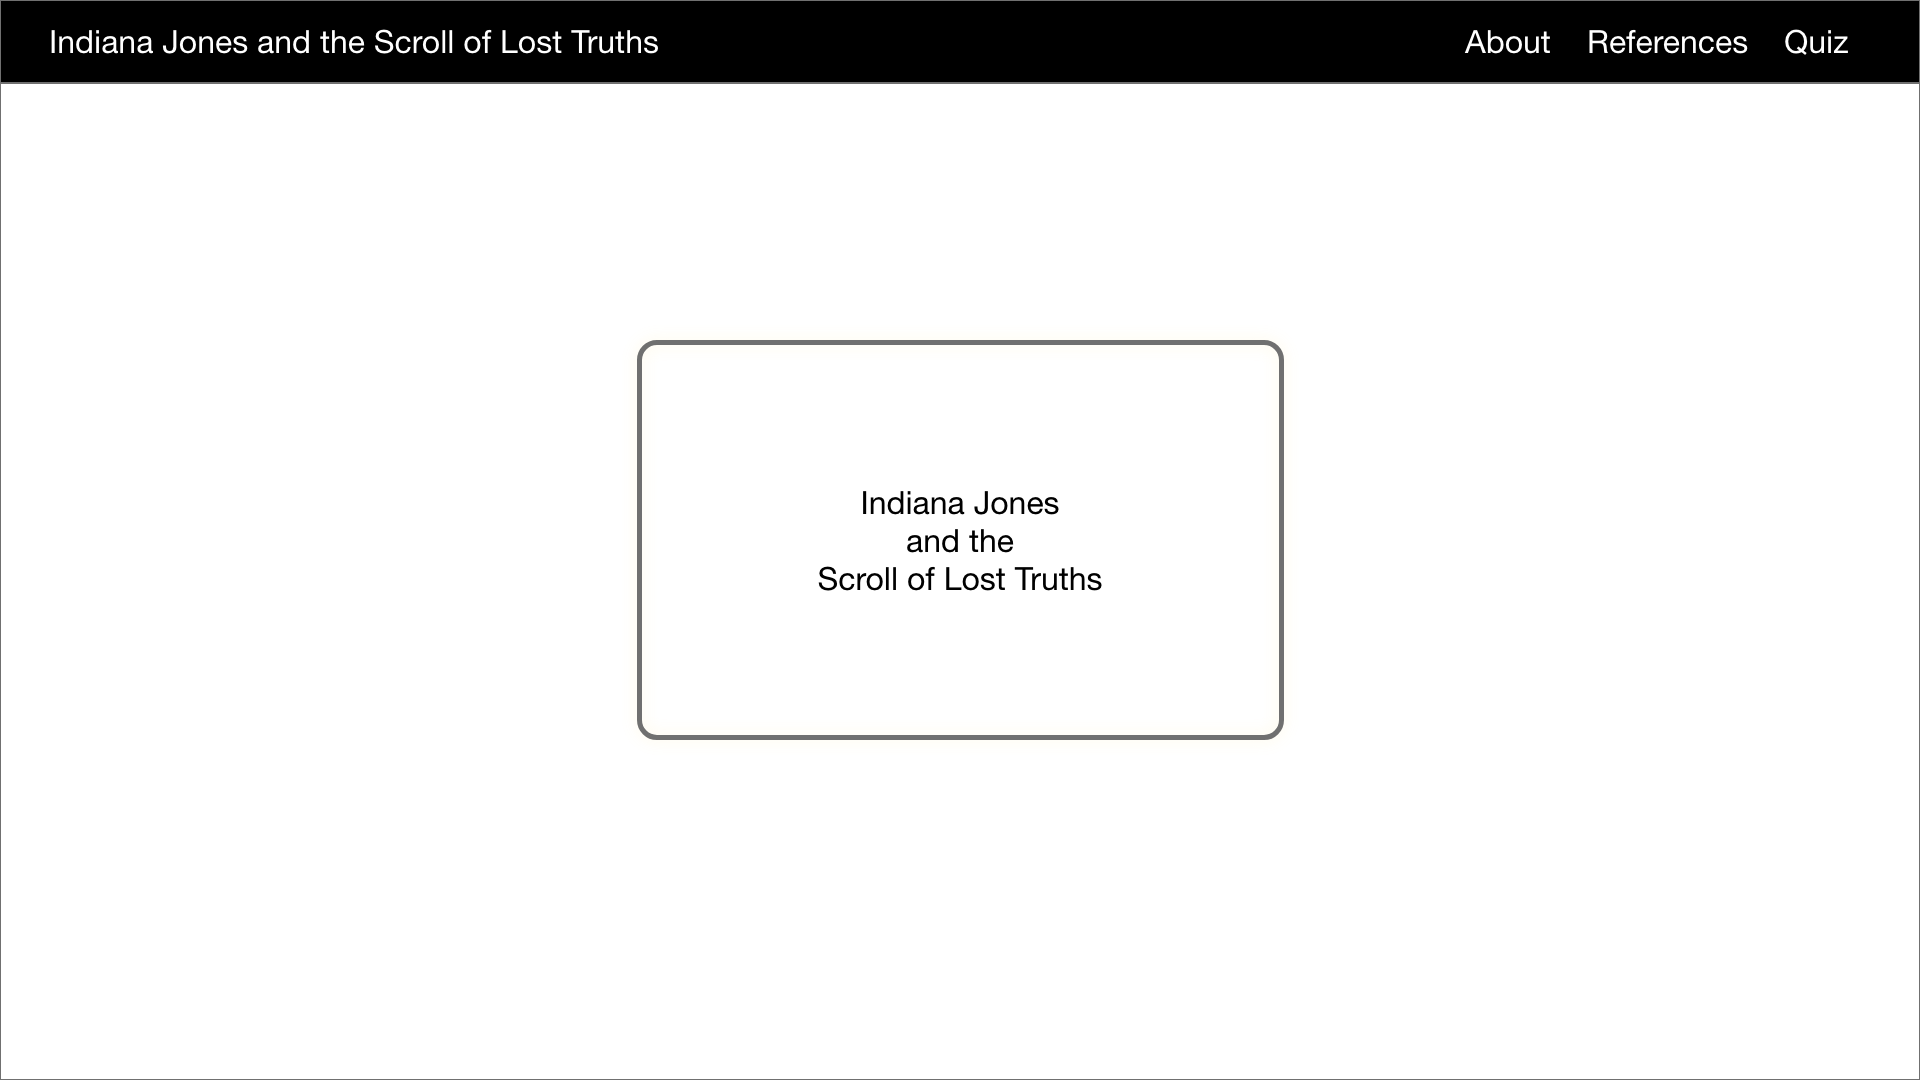
\includegraphics[width=0.9\linewidth]{wireframe/web1}	
	\caption{Wireframe mockup of main title page}\label{fig:wtitle}
\end{figure}
As shown in Figure~\ref{fig:wtitle}, the title page functions primarily as a welcome screen. The background will be an opening and inviting image, as well as set the scene for the wonders that will be covered in future visits. The overall aim of this screen therefore is to get people amazed and further interested in the content being presented. The title page will serve as the first screen and scrolling down will provide the content screens as covered in Section~\ref{sec:wcontent}.

\subsubsection{Main Content}\label{sec:wcontent}
\begin{figure}
	\centering
	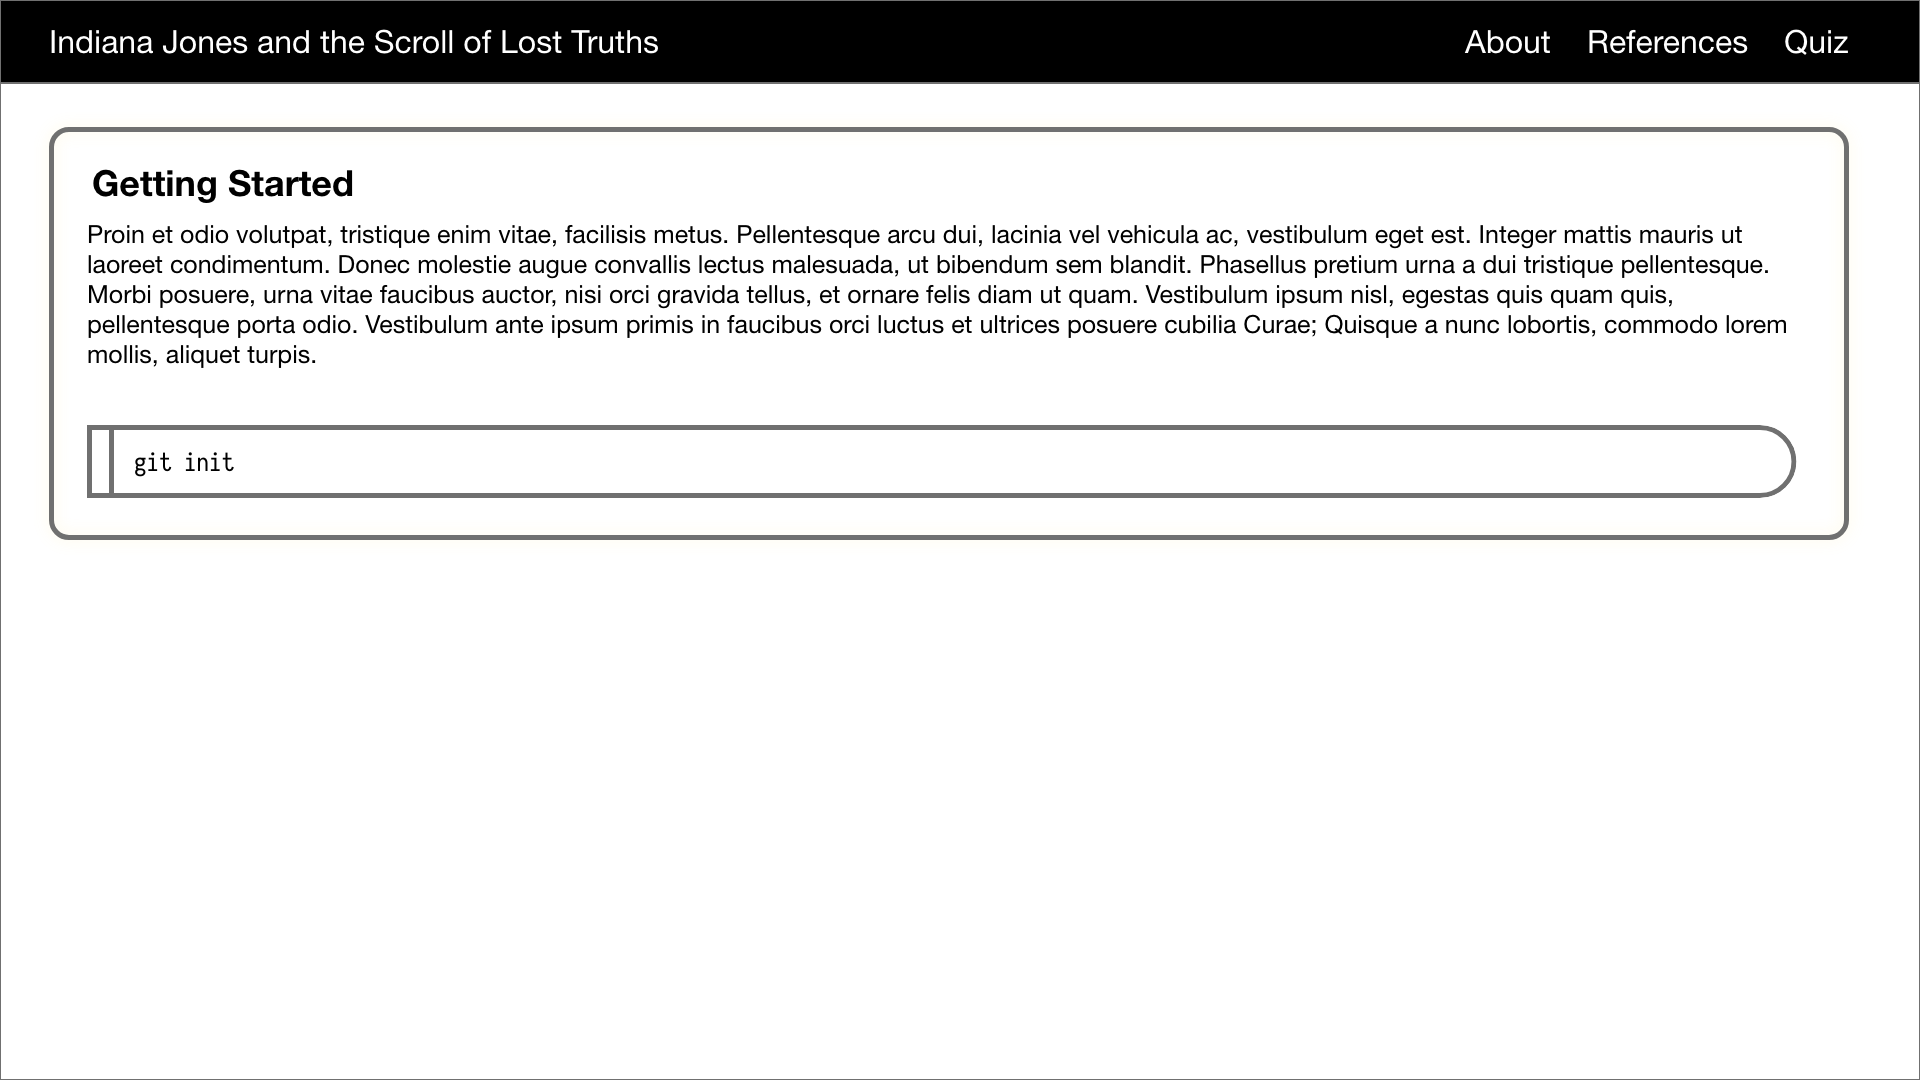
\includegraphics[width=0.9\linewidth]{wireframe/web2}	
	\caption{Wireframe mockup of single group of content}\label{fig:wcontent}
\end{figure}

\begin{figure}
	\centering
	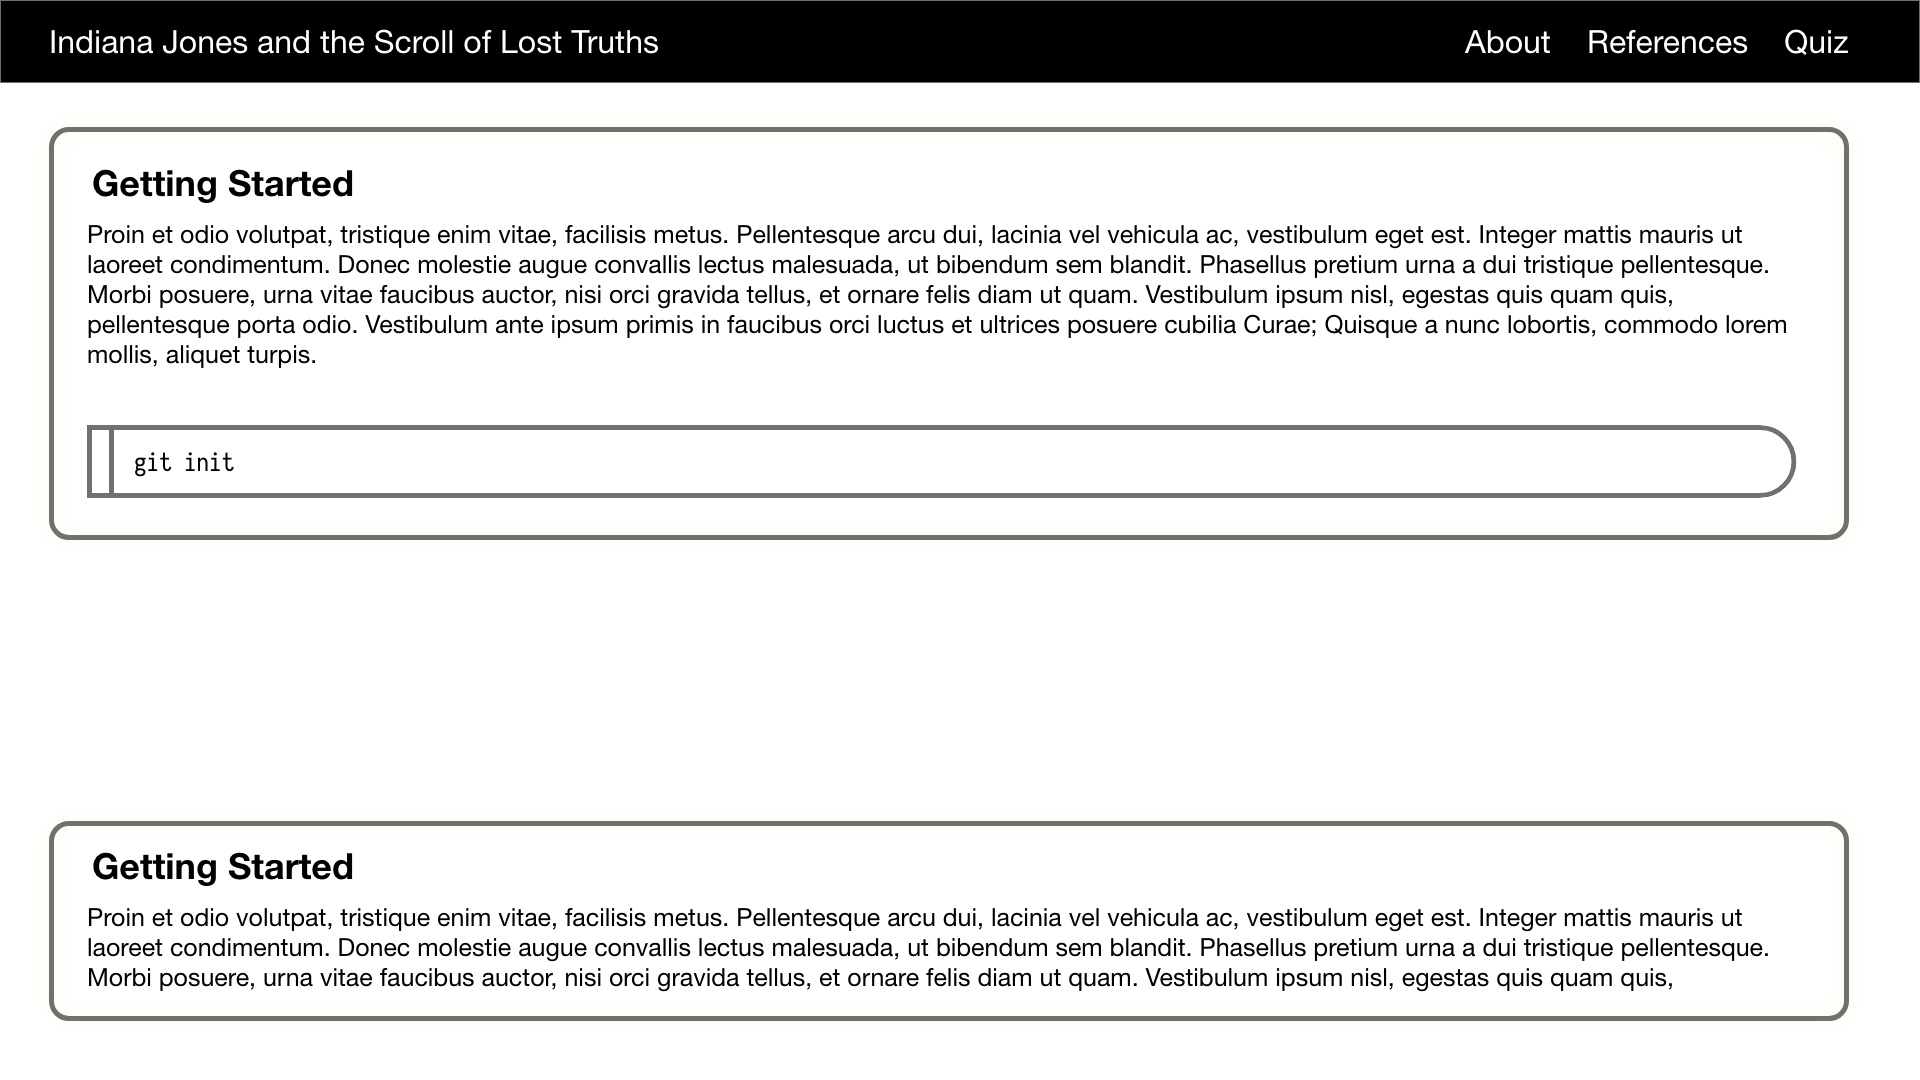
\includegraphics[width=0.9\linewidth]{wireframe/web3}
	\caption{Wireframe mockup of a page of content with two groups}\label{fig:wcontent2}
\end{figure}

The main content will be delivered using ``card''s, these cards will contain a header and some content as well as a background and rounded corners. Figure~\ref{fig:wcontent} shows the wireframe of a content screen with some reference command at the bottom of the card. A content page may also contain two cards (one anchored at the top, and one at the bottom), as shown in Figure~\ref{fig:wcontent2}.

\subsubsection{About}
\begin{figure}
	\centering
	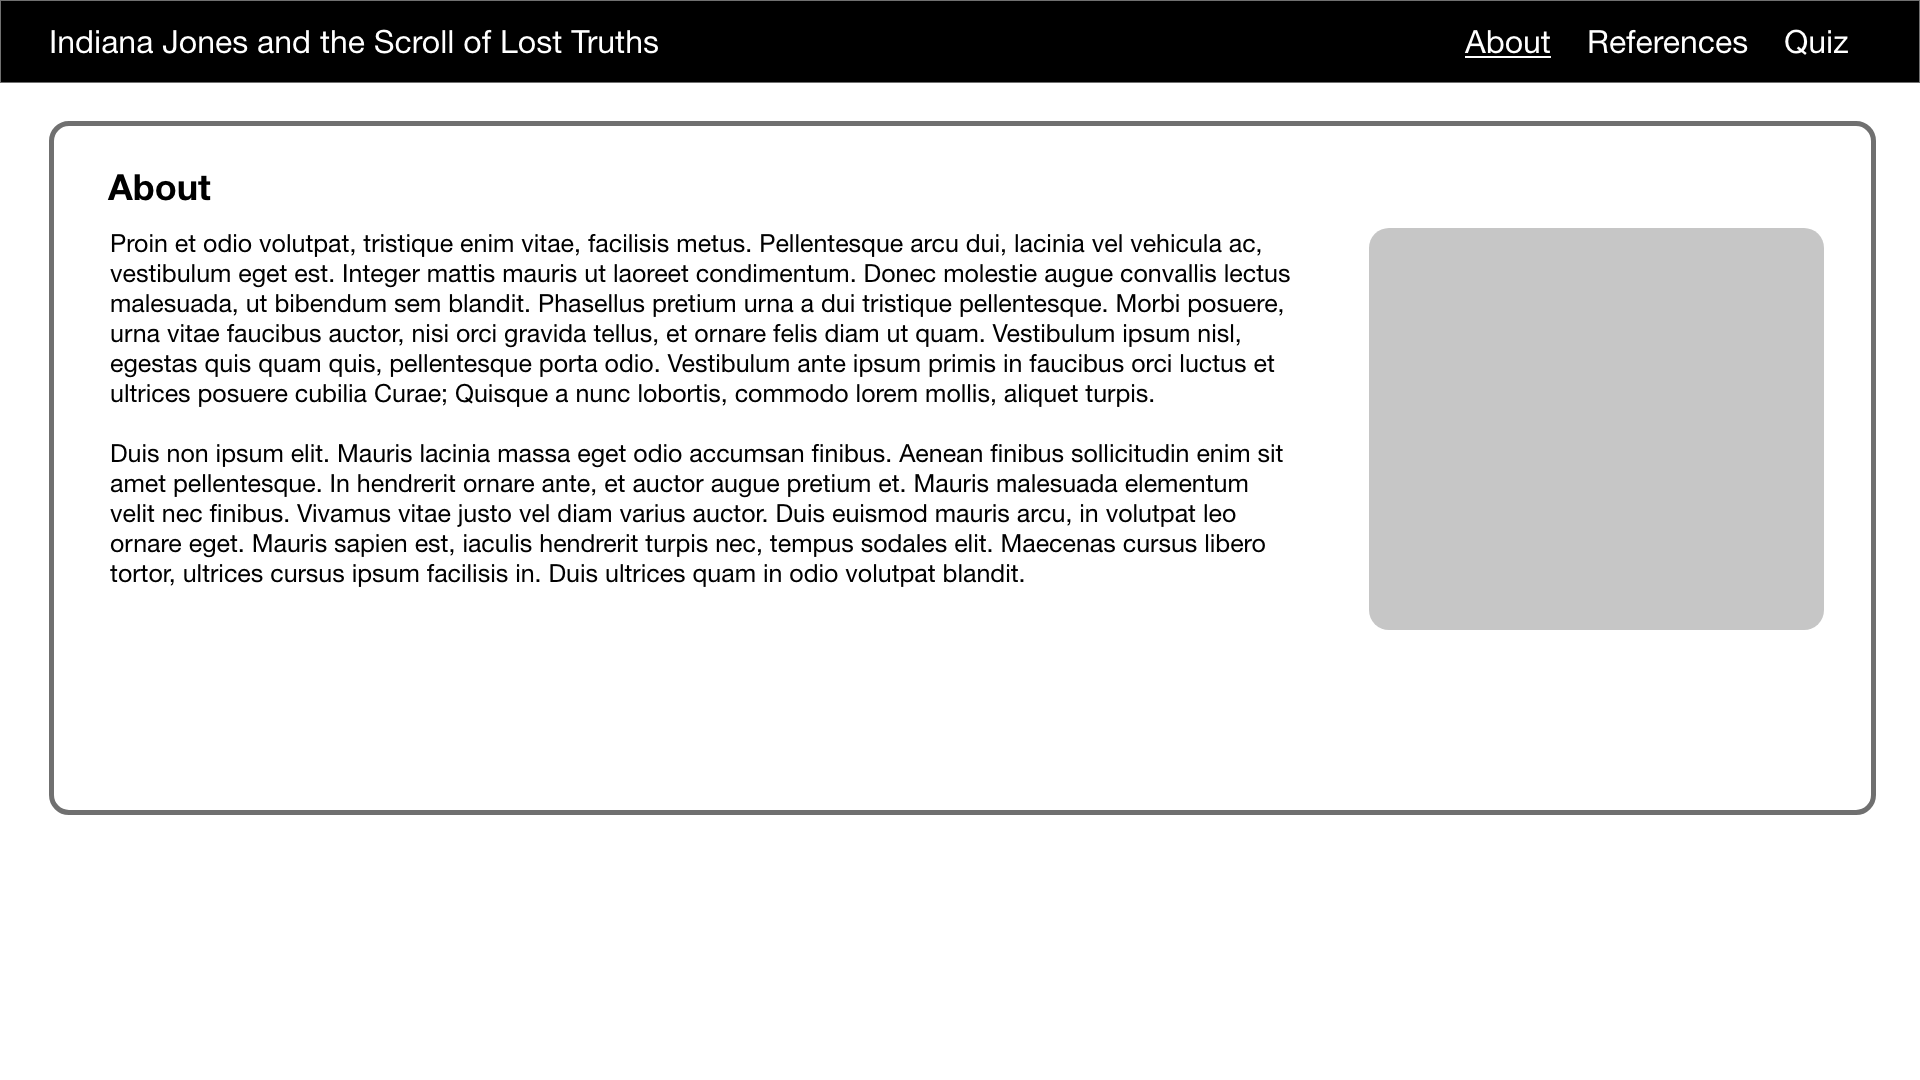
\includegraphics[width=0.9\linewidth]{wireframe/web4}
	\caption{Wireframe mockup of the about page}\label{fig:wabout}	
\end{figure}

The about page will be used as a way for people to find out information about the website and the author. Figure~\ref{fig:wabout} details the wireframe layout of the about page. The grey box on the right side will be used for a professional portrait photo of the author and the text on the side detailing both the author and the website. 

\subsubsection{References}
\begin{figure}
	\centering
	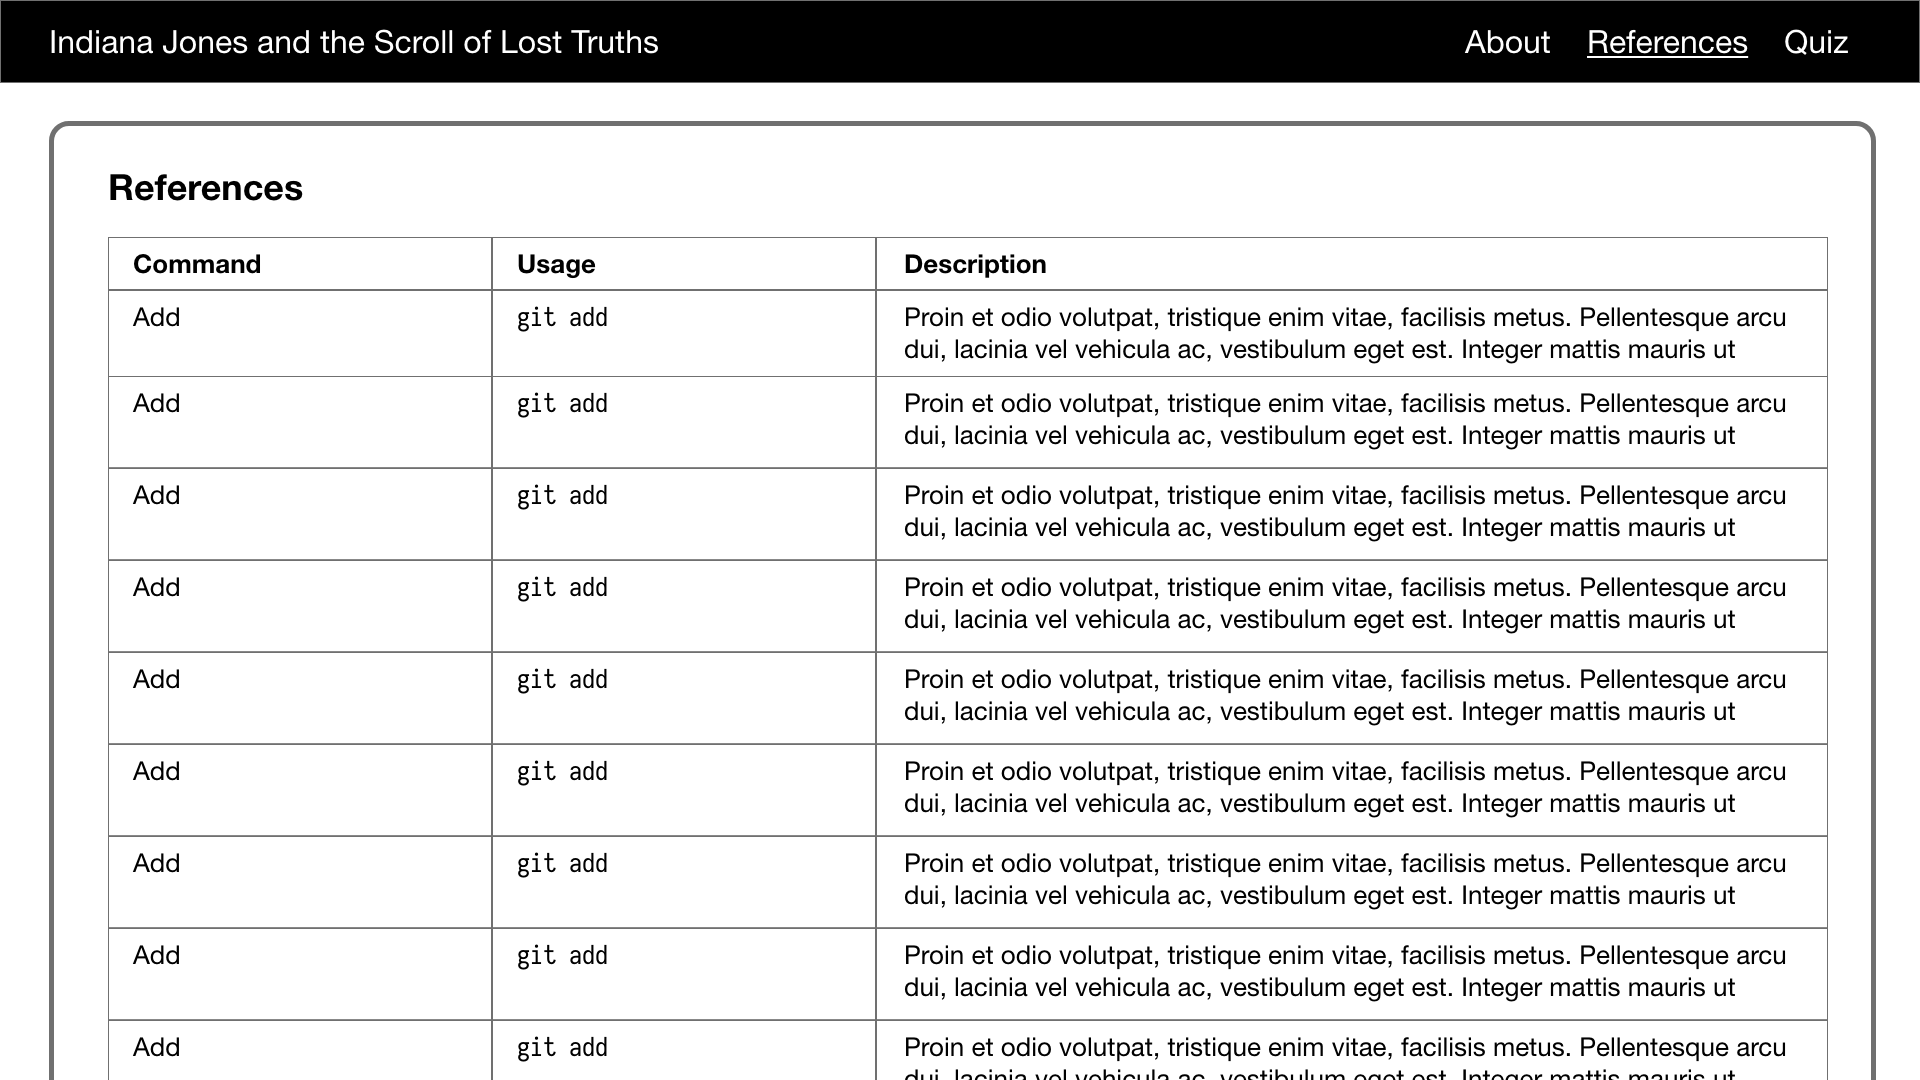
\includegraphics[width=0.9\linewidth]{wireframe/web5}
	\caption{Wireframe mockup of the references page}\label{fig:wreferences}	
\end{figure}

Figure~\ref{fig:wreferences} defines the wireframe for the references page. This page is the main page which users will go to for any quick information. Therefore most of the information regarding this page is placed into tables with a brief description in the rightmost column.

\subsubsection{Quiz}
\begin{figure}
	\centering
	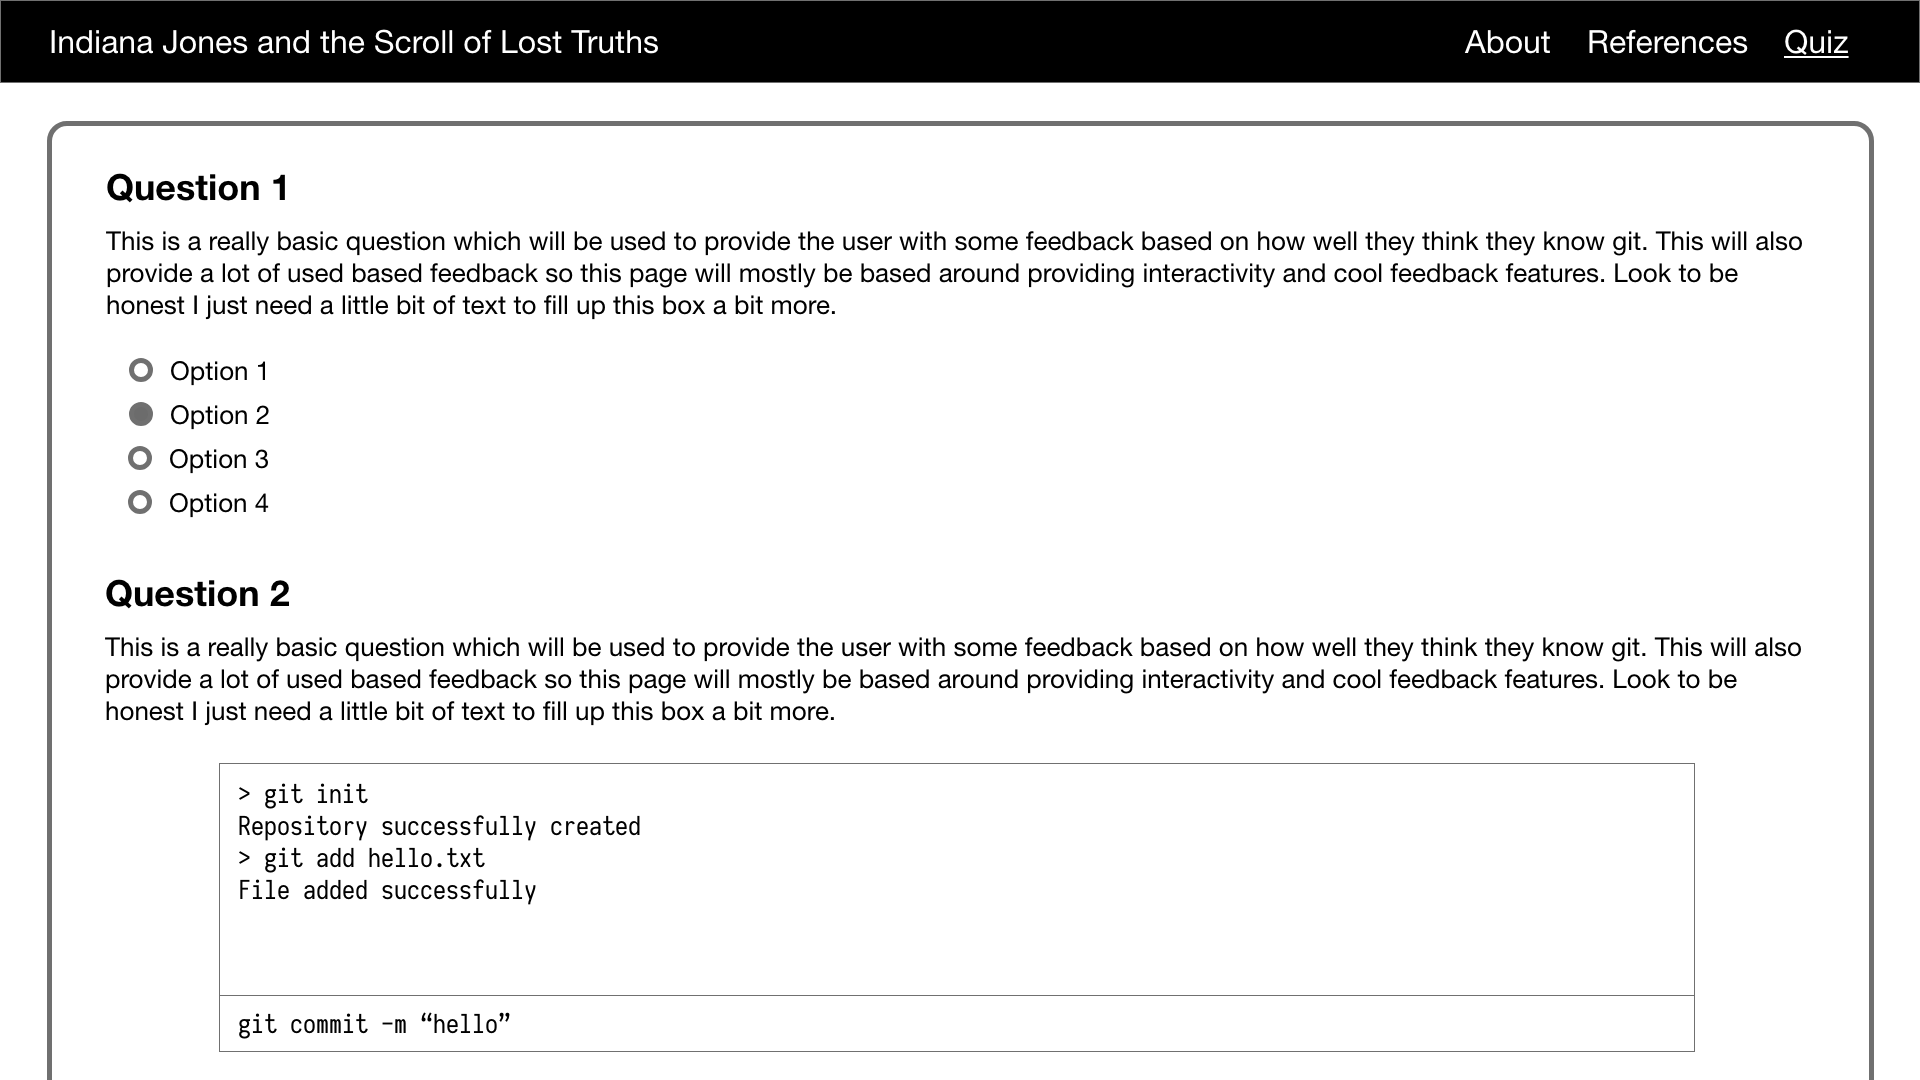
\includegraphics[width=0.9\linewidth]{wireframe/web6}
	\caption{Wireframe mockup of the quiz page}\label{fig:wquiz}	
\end{figure}

The quiz page will primarily be used for users to test themselves and their \gls{git} knowledge, this page will be focused heavily on user interaction and provide a lot of dynamic content. Figure~\ref{fig:wquiz} shows the wireframe with two interactive controls.\\\\
The first interactive control provides the user with the option to pick one option from a set of options. In Figure~\ref{fig:wquiz}, ``Option 2'' is selected as the users answer. Upon completion of the quiz, feedback will be provided locally to the control specifying if that particular answer is correct or incorrect.\\\\
The second interactive control allows the user to simulate using the \gls{git} commands in an emulated environment. Therefore they are able to enter different git commands and receive input based on these commands. Due to the amount of features provided with \gls{git}, not all commands will be implemented and only the set of commands covered in the main tutorial will be implemented. Upon completion of the quiz, if the result does not match the requested result from the question the user will be prompted to attempt this question again.


\subsection{Paper Prototyping}
% Reflect on the success of the Paper Prototyping design activity you did in Week 6
% Include photos/screenshots of your paper prototypes
% Include the testing plan you developed for the activity
% Include photos you took of the activity running
% What feedback did you get and how did it inform your visual organisation, navigation and functionality decisions?
\begin{figure}
	\centering
	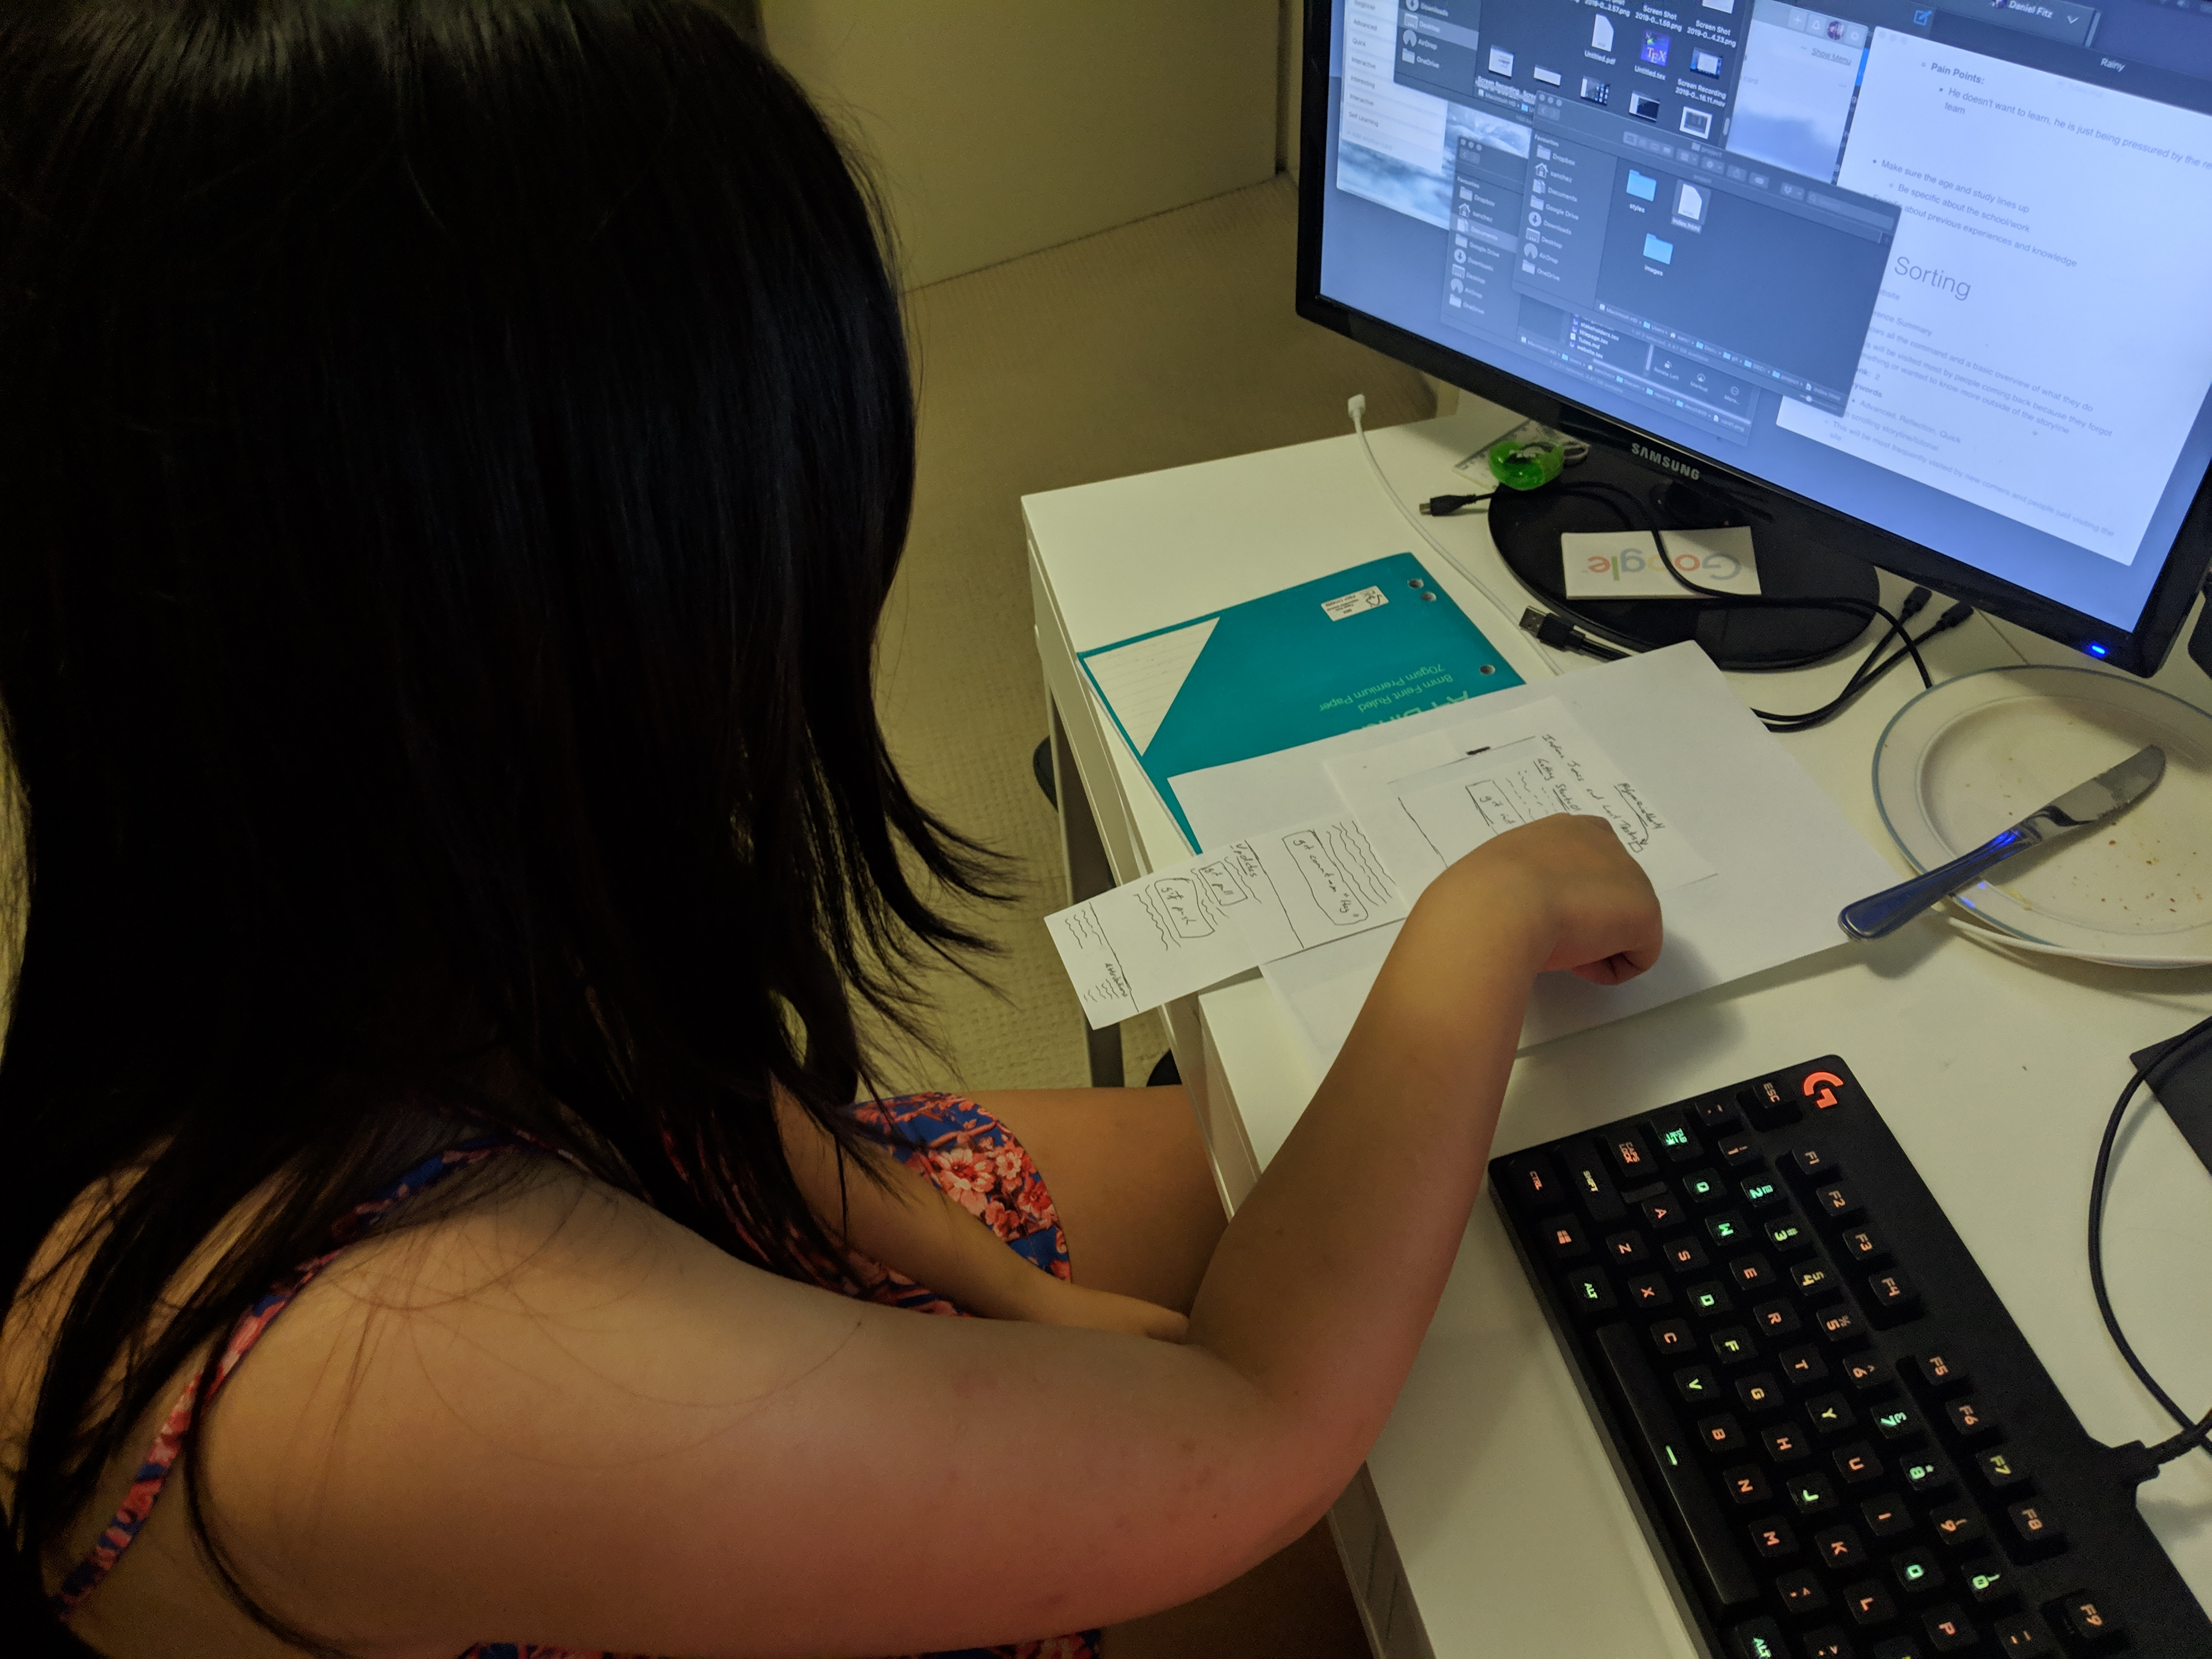
\includegraphics[width=0.8\linewidth]{rainy}
	\caption{User completing the paper prototype test}
\end{figure}

The paper prototype was broken up into the following tests:

\subsubsection{Learn the Basics}
\begin{itemize}
	\item\textbf{Do:} ``Learn the basics''
	\item\textbf{Watch:} If they scroll through the homepage or jump to references
	\begin{itemize}
		\item\textbf{Person 1:} Hovered over the code snippet. Hovered over the heading. ``Will I be looking at whitespace''
		\item\textbf{Person 2:} Went to the about page first
	\end{itemize}
	\item\textbf{Ask:}
	\begin{itemize}
		\item ``Was it intuitive to scroll	the page?''
		\begin{itemize}
			\item\textbf{Person 1:} Yeah very intuitive, but there is no menu have to scan the entire page
			\item\textbf{Person 2:} Yes it was quite intuitive, I think that normally when someone encounters a website they would scroll down for more information. Especially when the title says getting started
		\end{itemize}
		\item ``Do you feel like the content is will spaced out?''
		\begin{itemize}
			\item\textbf{Person 1:} Yeah but vertical spacing is verging on a little too much
			\item\textbf{Person 2:} If each section is separated then yes, otherwise separate pages might be effective
		\end{itemize}
	\end{itemize}
\end{itemize}


\subsubsection{Complete the Quiz}
\begin{itemize}
	\item\textbf{Do:} ``Complete the Quiz''
	\item\textbf{Watch:} How capable each of the controls in the quiz are
	\begin{itemize}
		\item\textbf{Person 1:} Got really confused about the terminal thing
	\end{itemize}
	\item\textbf{Ask:}
	\begin{itemize}
		\item ``Did you feel like it was obvious there was a quiz?''
		\begin{itemize}
			\item\textbf{Person 1:} Yeah it was obvious because of the quiz button. Weird it was between references and about
			\item\textbf{Person 2:} Yes because there was a heading up the top saying quiz
		\end{itemize}
		\item ``Was the Quiz easy to flow through?''
		\begin{itemize}
			\item\textbf{Person 1:} I don't know how many questions there are... Yes
			\item\textbf{Person 2:} Yes
		\end{itemize}
		\item ``Do you think you would benefit from the quiz?''
		\begin{itemize}
			\item\textbf{Person 1:} Yes cause I know what I don't know, find out weak spots
			\item\textbf{Person 2:} Yes because a quiz is useful to check whether the content learnt was absorbed
		\end{itemize}
	\end{itemize}	
\end{itemize}


\subsubsection{Get information on Advanced commands}
\begin{itemize}
	\item\textbf{Do:} ``Get information on Advanced commands''
	\item\textbf{Watch:} If they scroll through the home page screen first or go straight to the references page
	\begin{itemize}
		\item\textbf{Person 1:} Went to the homepage first
		\item\textbf{Person 2:} Went to the homepage first
	\end{itemize}
	\item\textbf{Ask:}
	\begin{itemize}
		\item ``Was it clear that there is a references overview page?''
		\begin{itemize}
			\item\textbf{Person 1:} Yeah but I thought it was citations, not git command references
			\item\textbf{Person 2:} Yes there was a title at the top saying references. Title it ``git command reference''
		\end{itemize}
	\end{itemize}	
\end{itemize}


\subsubsection{View information about the creator}
\begin{itemize}
	\item\textbf{Do:} ``View information about the site creator''
	\item\textbf{Watch:} How easy the navigation bar is to use
	\item\textbf{Ask:}
	\begin{itemize}
		\item ``Did you know exactly where you wanted to go?''
		\begin{itemize}
			\item\textbf{Person 1:} yeah but thought about was about the page not about the person
			\item\textbf{Person 2:} yes this was a very intuitive button
		\end{itemize}
	\end{itemize}	
\end{itemize}


\subsubsection{How do you update your git?}
\begin{itemize}
	\item\textbf{Do:} ``How do you update your git repo?''
	\item\textbf{Watch:} If they navigate to the references or the home page
	\begin{itemize}
		\item\textbf{Person 1:} Navigated to the home page
		\item\textbf{Person 2:} Navigated to the references page	
	\end{itemize}
	\item\textbf{Ask:}
	\begin{itemize}
		\item ``Did you know where you needed to go?''
		\begin{itemize}
			\item\textbf{Person 1:} Yeah I had a vague idea because I started on that page. I wouldn't if I didn't scroll the page
			\item\textbf{Person 2:} Yes, because the references will show me all the commands I can use
		\end{itemize}
	\end{itemize}	
\end{itemize}

\begin{figure}
	\centering
	\subfloat[Paper Prototype screen of the main homepage]{
		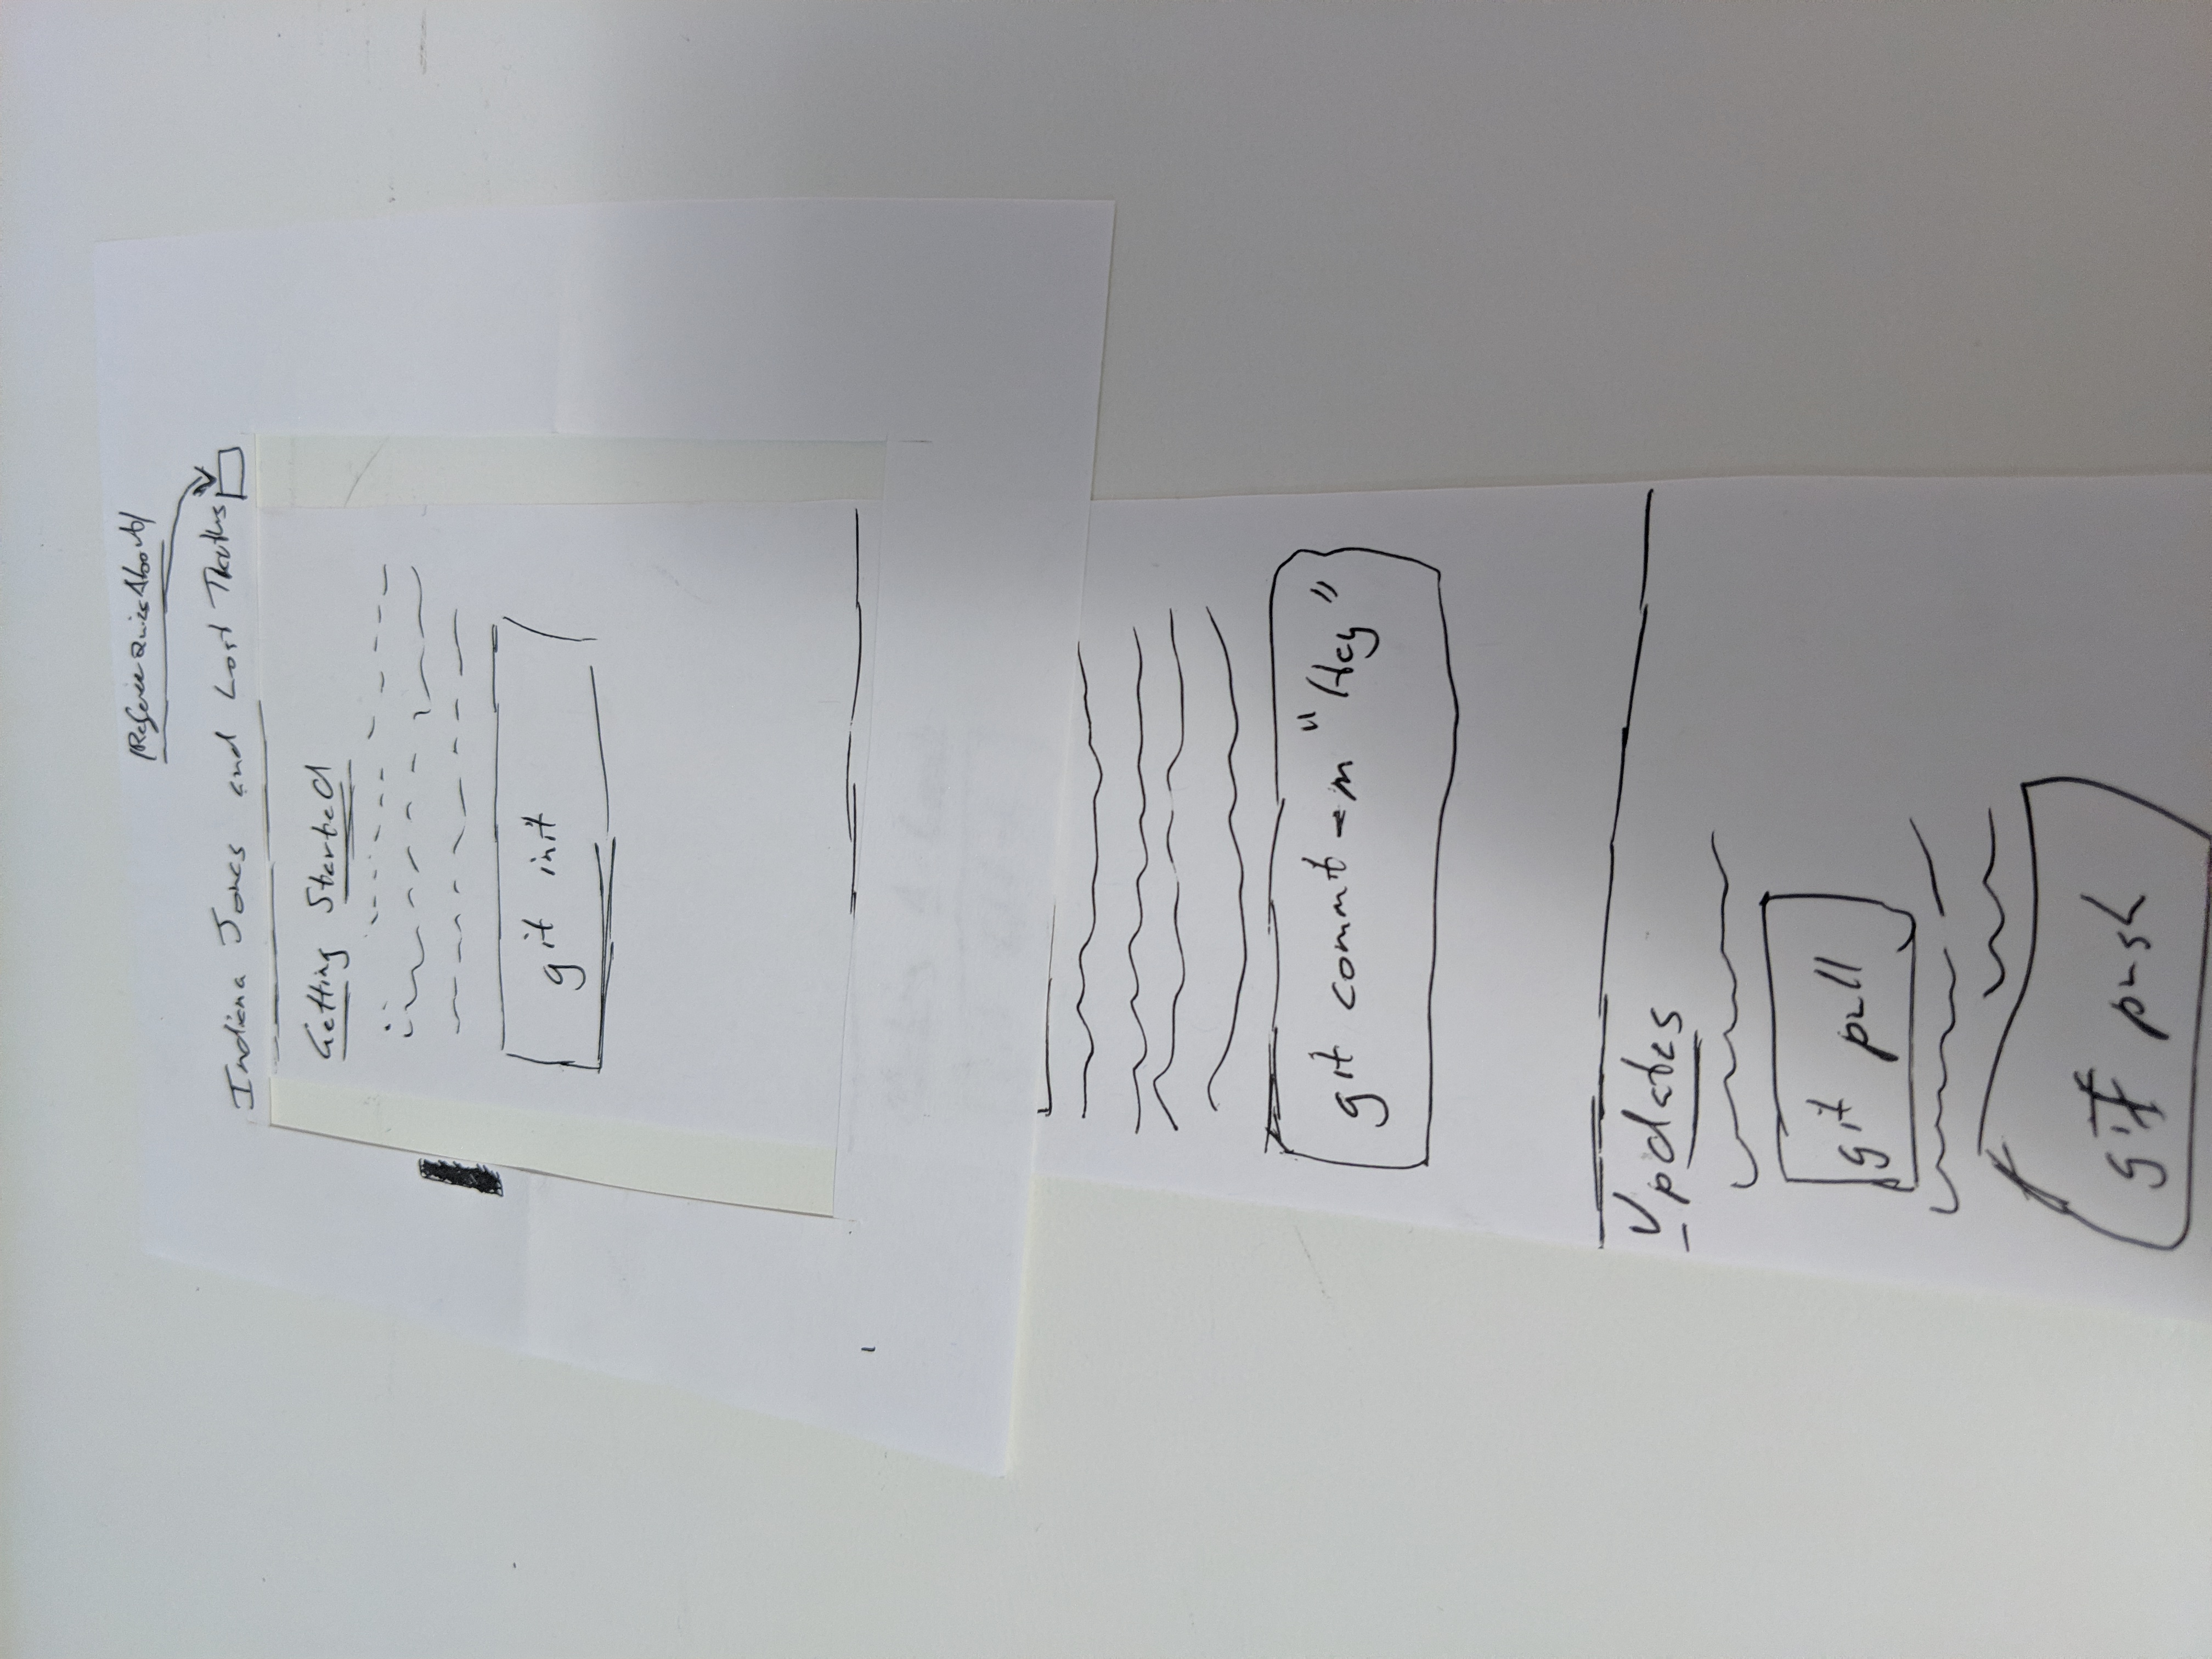
\includegraphics[width=0.5\textwidth,angle=-90,origin=c]{paper2}\label{fig:paper2}}
	\qquad
	\subfloat[Paper Prototype screen of the references page]{
		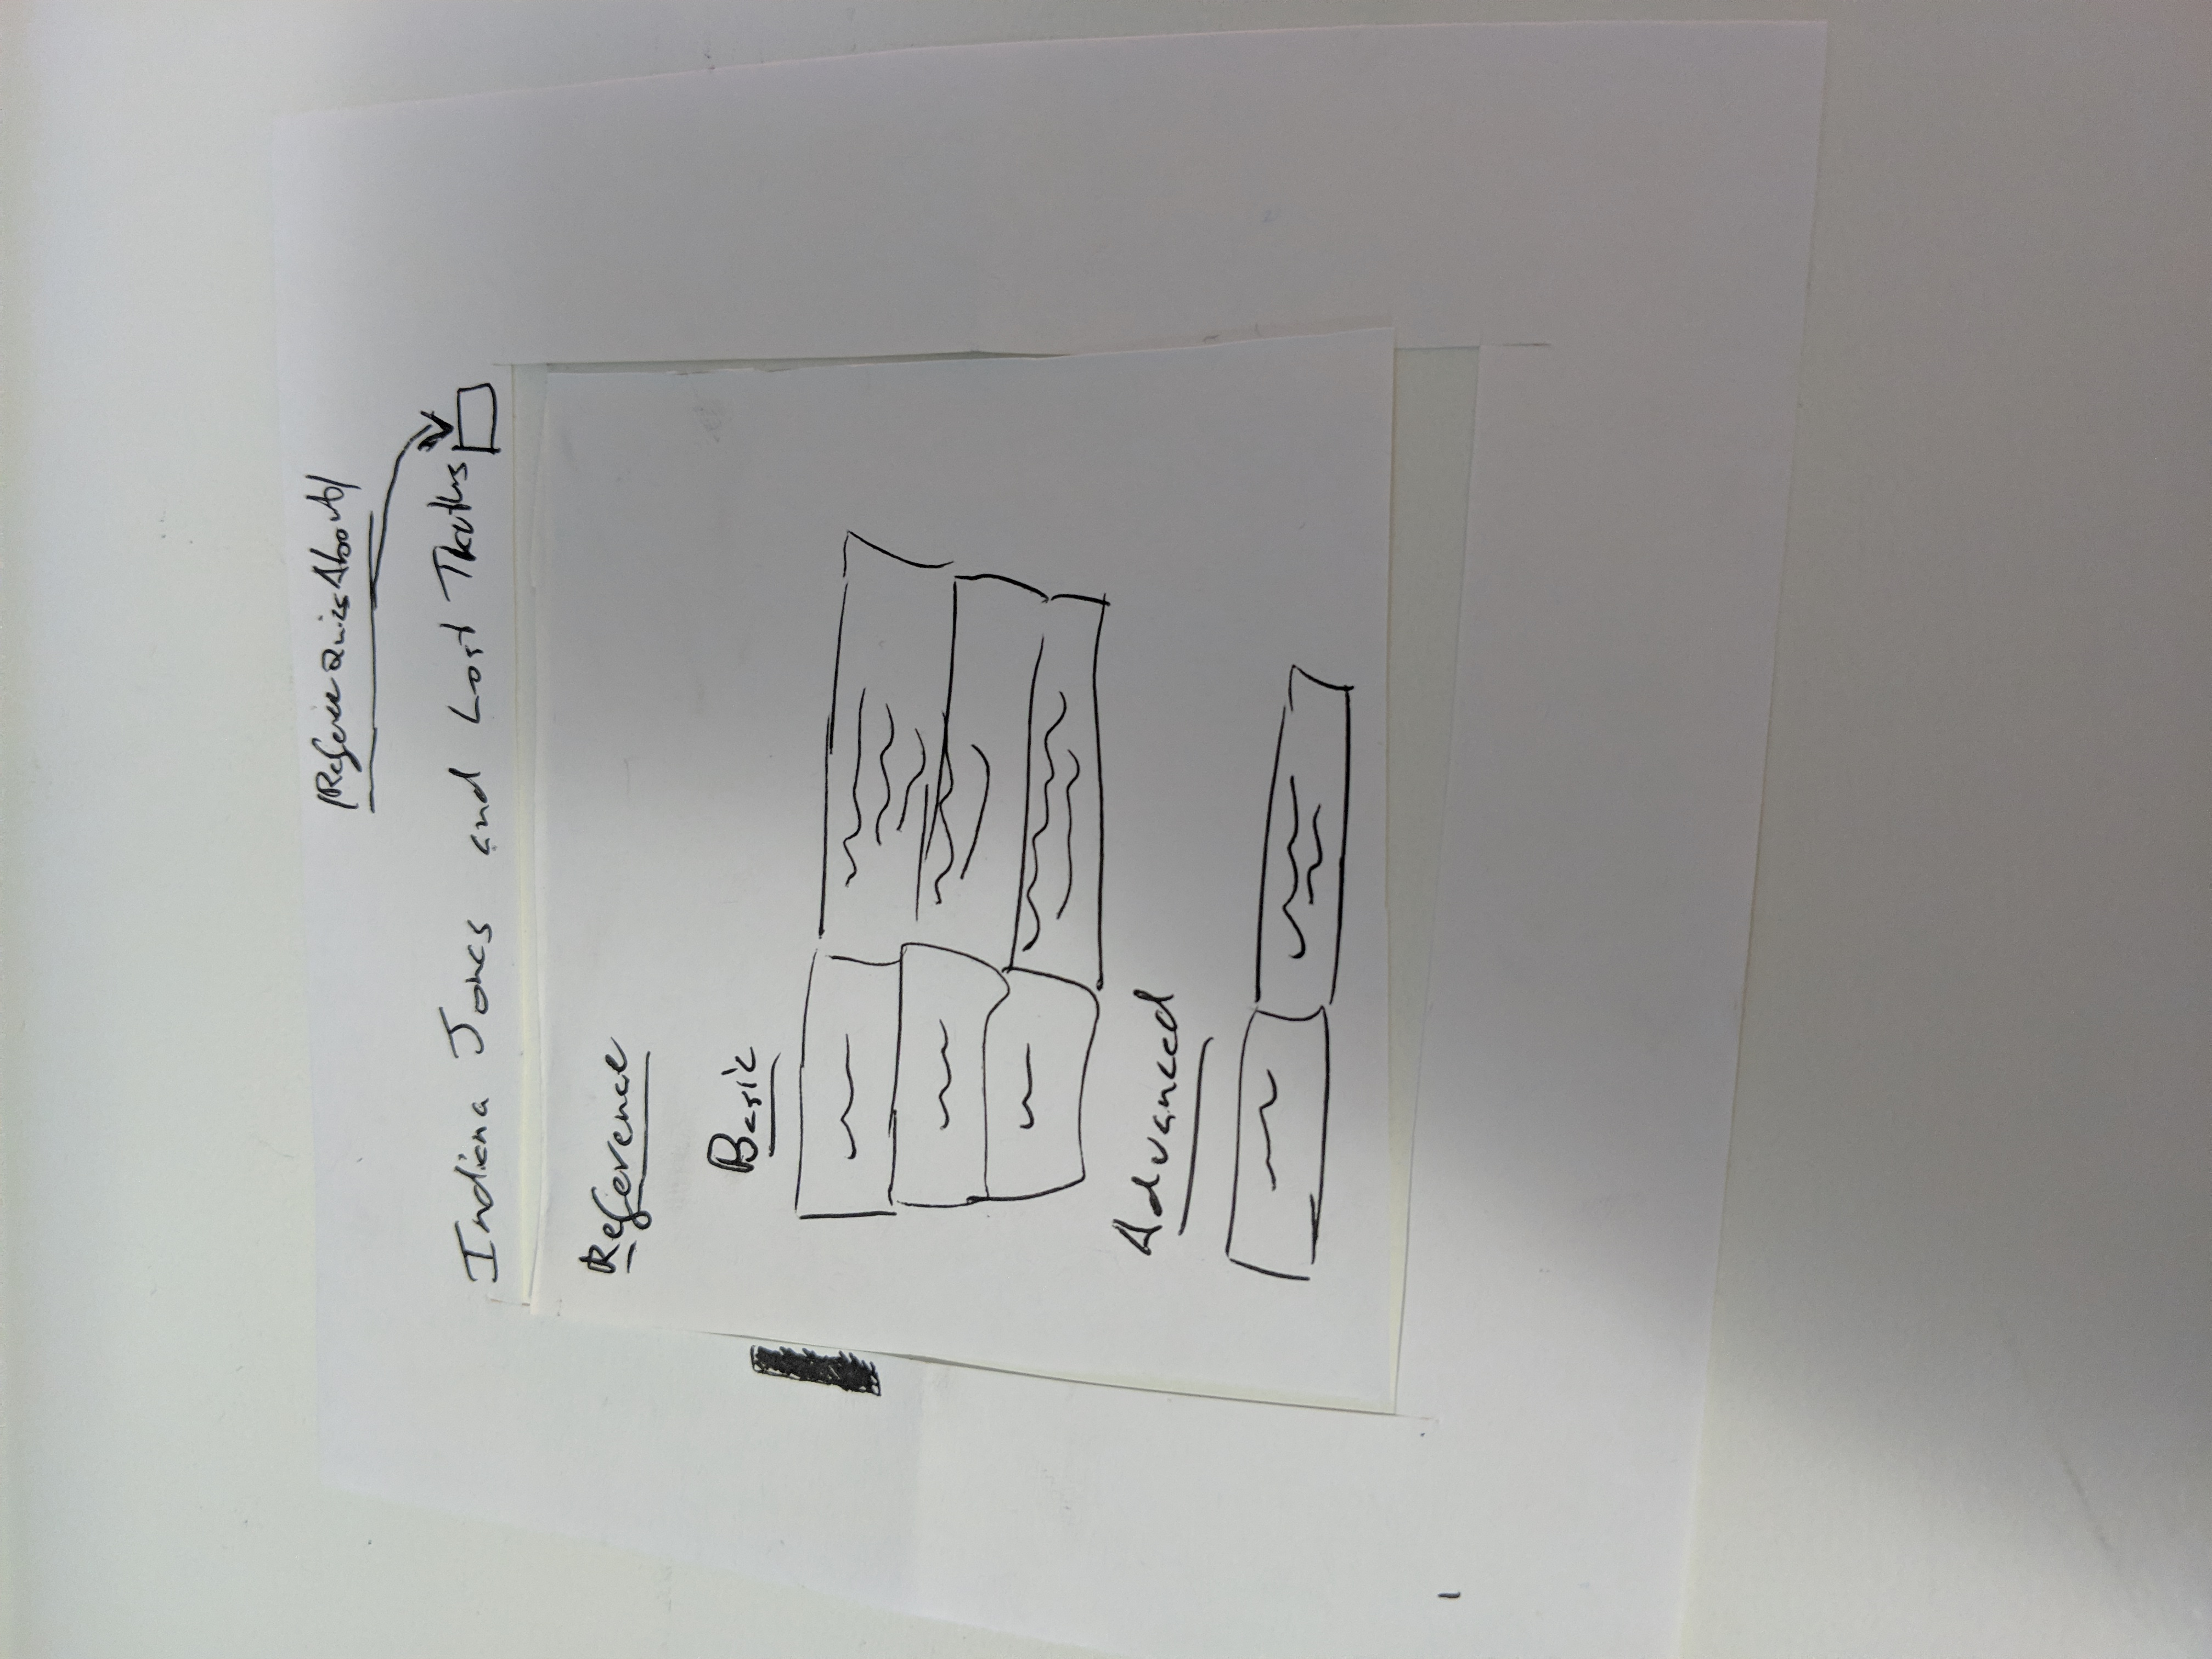
\includegraphics[width=0.5\textwidth,angle=-90,origin=c]{paper1}\label{fig:paper1}}

	\caption{Screenshots of paper prototype}
	\label{fig:paper}
\end{figure}

